
%(BEGIN_QUESTION)
% Copyright 2008, Tony R. Kuphaldt, released under the Creative Commons Attribution License (v 1.0)
% This means you may do almost anything with this work of mine, so long as you give me proper credit

Tegn nødvendige koblinger for å få denne trykkbryteren til å styre lampene på følgende måte. 

\begin{itemize}
\item{} Høyt prosesstrykk: grønt lys på og rødt av.
\item{} Lavt prosesstrykk: rødt lys på og grønt lys av.
\end{itemize}

$$\includegraphics[width=15.5cm]{i03251x01.eps}$$

Hint: remember that the ``normal'' status of a switch is defined as the status of {\it minimum stimulus}: when the switch is exposed to the lowest possible degree of process stimulation (in this particular case, to the lowest possible pressure).

\underbar{file i03251}
%(END_QUESTION)





%(BEGIN_ANSWER)

This is just one possible solution:

$$\includegraphics[width=15.5cm]{i03251x02.eps}$$
 
%(END_ANSWER)





%(BEGIN_NOTES)


%INDEX% Pictorial circuit review (process switch circuit)

%(END_NOTES)


